%!TEX root = ../thesis.tex
%*******************************************************************************
%*********************************** First Chapter *****************************
%*******************************************************************************

\chapter{Introduction} \label{sec:intro}

\ifpdf
    \graphicspath{{Chapter1/Figs/Raster/}{Chapter1/Figs/PDF/}{Chapter1/Figs/}}
\else
    \graphicspath{{Chapter1/Figs/Vector/}{Chapter1/Figs/}}
\fi

\section{DNA methylation} \label{sec:intro_met}

Epigenetics is the study of heritable changes of gene activity that cannot be explained by changes of the DNA sequence itself~\citep{holliday_dna_1996}. Epigenetic factors include DNA methylation, histone modifications, and small non-coding RNA sequences. The modification of histone proteins by methylation, acetylation, or ubiquitination influences DNA accessibility and thereby gene expression. Small RNA sequences, such as miRNAs, can bind to the RNA of a target gene and thereby silence gene expression. The focus of this thesis is on DNA methylation, a chemical modification of cytosine to 5-methylcytosine (5mC) by the attachment of a methyl group to the fifth carbon atom of cytosine (\Cref{fig:intro_cpg}).  DNA methylation mainly occurs at CpG sites, i.e. cytosine nucleotides that are followed by a guanine nucleotide. CpG sites are underrepresented in the genome since they are `mutational hotspots': 5mC is prone to be deaminated to thymine, resulting in a C$\rightarrow$T mutation. CpG sites therefore cluster into CpG islands (CGIs), which are characterized by a GC density above 50\%. CpG methylation plays an important role in biology, including gene regulation, imprinting, X-chromosome inactivation, and the repression of retroviruses~\citep{holliday_dna_1996,robertson_dna_2005,jones_functions_2012,moore_dna_2013}.

\begin{figure}[htbp!]
\centering
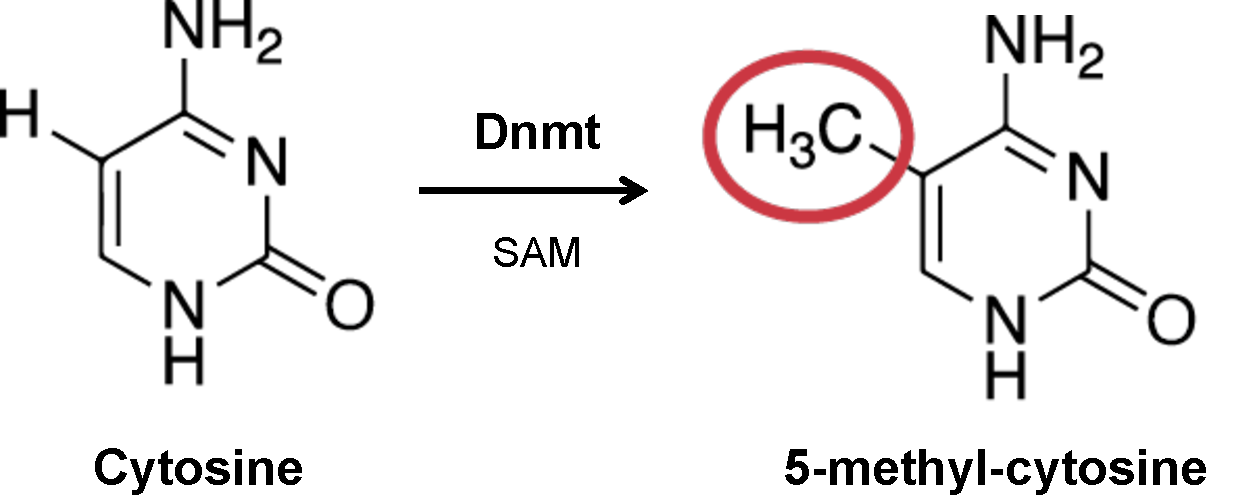
\includegraphics[width=0.7\textwidth]{cpg}
\caption[Chemical reaction of cytosine to 5-methylcytosine.]{Chemical reaction of cytosine to 5-methylcytosine. Cytosine is converted to 5-methylcytosine (5mC) by the transfer of a methyl group from S-adenosyl-L-methionine (SAM) to the fifth carbon atom of the cytosine pyrimidine ring, catalyzed by enzymes of the DNA methyltransferase (Dnmt) family.}
\label{fig:intro_cpg}
\end{figure}

DNA methylation can also occur at non-CpG sites, including CHG and CHH sites, where H can be any nucleotide except for G. Non-CpG methylation has been reported in plants, fungi, and embryonic stem cells (ESCs), but the functional relevance of non-CpG methylation is still unclear~\citep{jones_functions_2012,ziller_genomic_2011,ramsahoye_non-cpg_2000,shirane_mouse_2013}.

DNA methylation is established during embryonic development by a series of de novo methylation and demethylation events. Enzymes of the DNA methyltransferase (Dnmt) family catalyse DNA methylation by transferring the methyl-group of S-adenosyl-L-methionine (SAM) to cytosine (\Cref{fig:intro_cpg}). Three active Dnmt enzymes have been identified in mammals: Dnmt1, Dnmt3a, and Dnmt3b. Although these enzymes are structurally similar, they serve different functions and are expressed at different time points during embryonic development~\citep{moore_dna_2013,jones_rethinking_2009,bestor_notes_2015}. Dnmt3a and Dnmt3b are also known as \emph{de novo Dnmts} since they establish new tissue-specific methylation patterns during embryogenesis (\Cref{fig:intro_dnmt}~(a)). Whereas Dnmt3a is ubiquitously expressed in all cell types, Dnmt3b is only expressed in differentiating cells. Dnmt1 is also known as \emph{maintenance Dnmt} since it maintains DNA methylation during cell division and cell differentiation. Dnmt1 preferentially binds to hemimethylated DNA during DNA replication, and methylates cytosine residues on the newly synthesized DNA strand (\Cref{fig:intro_dnmt}~(b)). Dnmt1 regulates genomic imprinting by repressing either the maternal or paternal copy of genes, and is involved in DNA repair.

\begin{figure}[htbp!]
  \begin{minipage}[c]{0.62\textwidth}
    \centering
    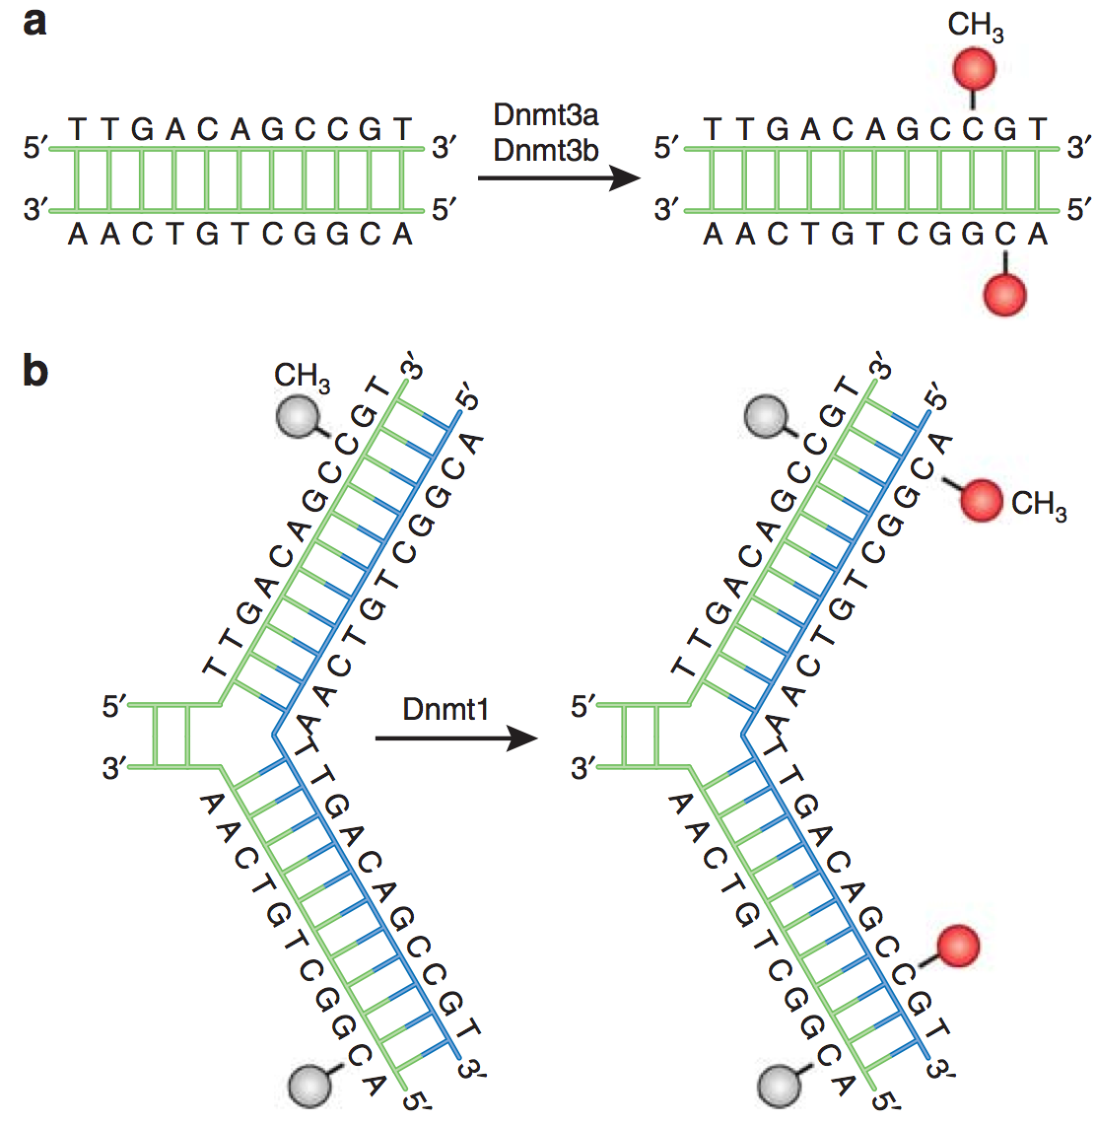
\includegraphics[width=0.9\textwidth]{dnmt}
  \end{minipage}
  \begin{minipage}[c]{0.36\textwidth}
    \caption[DNA methyltransferase enzymes.]{DNA methyltransferase enzymes. DNA methyltransferase (Dnmt) is a family of enzymes that catalyzes the conversion from cytosine to 5-methylcytosine. (a) Dnmt3a and Dnmt3b can establish new methylation patterns by methylating DNA de novo. (b) Dnmt1 maintains existing methylation patterns during cell replication by methylating hemimethylated DNA. It binds close to the replication fork and methylates CpG sites on the newly synthesized daughter strand at CpG sites that are methylated on the parent strand. Source: \citet{moore_dna_2013}.}
    \label{fig:intro_dnmt}
  \end{minipage}
\end{figure}

Although DNA methylation is primarily established during embryonic development and maintained in replicating cells, methylation patterns can be changed by environmental factors and stochastic fluctuations. DNA methylation can be erased passively by the inhibition of Dnmt1, resulting in gradually decreasing methylation levels in differentiating cells. Active demethylation can occur in both differentiating and non-differentiating cells, which involves the removal of the methyl group from 5mC through are series of chemical reactions~\citep{mayer_embryogenesis:_2000,zhang_active_2007}.

\section{Functions of DNA methylation} \label{sec:intro_fun}

The function of DNA methylation varies between genomic contexts~\citep{bestor_notes_2015,moore_dna_2013,jones_functions_2012,bird_dna_2002}. Promoter methylation has been associated with regulatory effects on gene expression~\citep{moore_dna_2013,jones_functions_2012,bird_dna_2002}. About 70\% of all promoters in the human genome are CGI promoters, i.e. promoters that are overlapped by at least one CGI. Promoter CGIs are evolutionary conserved, which indicates their functional importance. Most promoter CGIs are unmethylated and nucleosome depleted, which has been associated with increased DNA accessibility and gene expression levels~\citep{moore_dna_2013}. The high GC density in CGI promoters has further been associated with an increased binding of transcription factors that regulate gene expression~\citep{moore_dna_2013}. Methylation of promoter CGIs blocks RNA polymerases and thus inhibits gene expression. This is important to variably activate and deactivate genes during cell differentiation and to establish tissue-specific expression patterns in combination with other epigenetic factors. CGI promoter methylation further regulates imprinting by inhibiting the expression of either the maternal or paternal allele of genes. Another import role of CGI promoter methylation is X chromosome inactivation—the deactivation of one copy of the X chromosome in female mammalian cells by bulk methylation of all gene promoters~\citep{bestor_notes_2015}.

Unlike CGI promoters, which are predominantly unmethylated, non-CGI promoters are more heterogeneous. Although evidence exists that non-CGI promoter methylation may be involved in tissue-specific gene regulation~\citep{moore_dna_2013,jones_functions_2012}, the exact regulatory mechanisms are still unknown.

Intergenic regions are CpG poor and tend to be methylated. Methylation of intergenic regions is important for repressing transposable and viral elements~\citep{moore_dna_2013,jones_functions_2012,robertson_dna_2005}, which account for about 45\% of the genomic DNA in mammalian cells. These elements are either repressed by CpG methylation or inactive due to C$\rightarrow$T mutations acquired by the spontaneous deamination of 5mC. For example, the intracisternal A-particle (IAP) is a detrimental retrovirus that resides in the mouse genome~\citep{walsh_cytosine_1999}. IAPs are highly methylated by Dnmt1 and thereby repressed. Knockout of Dnmt1 induces demethylation and hence the expression and IAPs and cell death~\citep{walsh_cytosine_1999,hutnick_repression_2010}.

Gene bodies are CpG poor and mostly methylated, similar to intergenetic regions. Gene body methylation likewise serves as a mechanism to repress transposable and viral elements~\citep{moore_dna_2013,jones_functions_2012,robertson_dna_2005}. Although gene bodies are generally CpG poor, they can contain CGIs. However, methylation of gene body CGIs does not block transcription, unlike promoter CGIs, and the implications of gene body methylation in gene regulation is still unclear: Whereas some studies found positive associations between gene body methylation and gene expression, others have reported negative associations in slowly dividing and non-dividing cells.

Gene enhancers are relatively short (50-1500~bp) genetic elements that promote gene expression~\citep{blackwood_going_1998,pennacchio_enhancers:_2013}. They tend to be GC poor and to have heterogeneous methylation levels. For example, low methylated regions (LMRs~\citep{stadler_dna-binding_2011}) are indicative of distal enhancer elements. They are characterized by an average methylation rate of 30\%, which can fluctuate considerably during cell differentiation. Although some studies found negative associations between enhancer methylation and gene expression, further studies are needed to explore the regulatory function of these associations.

Insulators are genetic elements that block promoter-enhancer interactions~\citep{burgess-beusse_insulation_2002}. Insulators are bound by the CTCF zinc finger protein and transported close to gene promoters by looping of the DNA strand. Insulator methylation can block CTCF binding, and thereby support promoter-enhancer interactions. However, the roles of insulator methylation are still unclear~\citep{moore_dna_2013,jones_functions_2012}.

\section{Protocols for methylation profiling} \label{sec:intro_proto}

Several methods have been developed for profiling DNA methylation, which can be broadly grouped into protocols based on enzymatic digestion, affinity enrichment, and bisulfite conversion~\citep{yong_profiling_2016,schwartzman_single-cell_2015,plongthongkum_advances_2014,huang_profiling_2010,laird_principles_2010-1}.

\begin{figure}[htbp!]
\centering
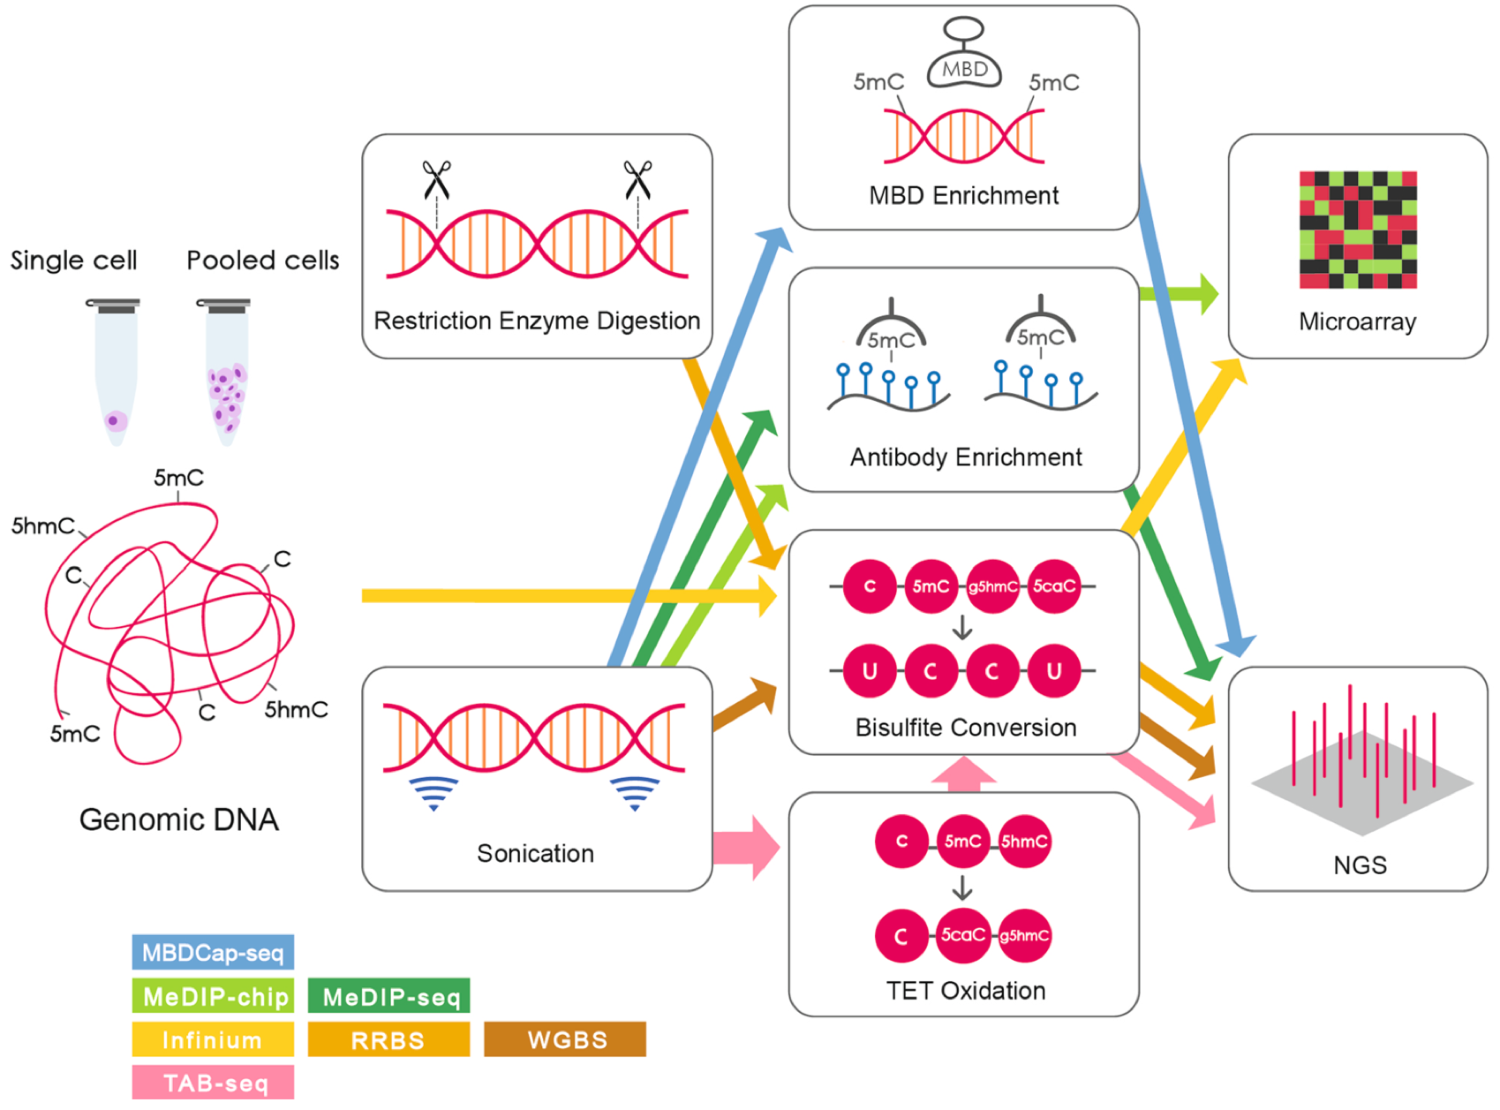
\includegraphics[width=0.8\textwidth]{seq}
\caption[Workflow of DNA methylation profiling protocols.]{Workflow of DNA methylation profiling protocols. DNA starting material is extracted from either a bulk population of cells or a single cell and fragmented by enzymatic digestion or sonication. Enrichment based profiling protocols enrich for methylated DNA fragments by either methyl-binding domain (MBD) proteins or antibodies. Bisulfite conversion-based protocols treat DNA fragments by bisulfite to convert unmethylated cytosine to thymine. DNA methylation levels are quantified by microarray hybridization of next generation sequencing (NGS). Source: \citet{yong_profiling_2016}.}
\label{fig:intro_seq}
\end{figure}

Protocols based on enzymatic digestion leverage methylation-sensitive restriction enzymes (MREs), which have differential digestion properties for methylated and unmethylated CpG sites. The two most common MREs are HpaII, which cleaves unmethylated CpG sites, and Msp1, which cleaves methylated CpG sites. Protocols proceed by enzymatically digesting DNA using a specific MRE, followed by DNA methylation quantification using either array hybridization (MRE-chip~\citep{chittur_help_2010}) or sequencing (MRE-seq~\citep{maunakea_conserved_2010}). Enzymatic digestion-based approaches are cost-effective and enable genome-wide methylation profiling. However, their resolution is limited to regions adjacent to MRE recognition sites, and they cannot quantify the methylation level of single CpG sites.

Affinity enrichment-based protocols enrich for methylated DNA fragments by either methyl-binding domain (MBD) proteins or antibodies that target 5mC. Methylated DNA immunoprecipitation (MeDIP) uses anti-methylcytosine antibodies to bind and quantify 5mC. The protocol consists of DNA fragmentation by sonication, enrichment of methylated fragments by immunoprecipitation, and methylation quantification by either array hybridization (MeDIP-chip~\citep{park-sarge_methylated_2009}) or sequencing (MeDIP-seq~\citep{brinkman_whole-genome_2010}). MeDIP is cost effective and can differentiate between CpG, CHG, and CHH methylation contexts. Since MeDIP only requires small amounts of DNA starting material, it is further applicable to small cell populations. On the downside, the resolution of MeDIP is limited to 100-300~bp long fragments and the method is biased towards hypermethylated regions.

Protocols based on bisulfite conversion enable quantifying the methylation levels of single CpG sites. In bisulfite conversion-based protocols, DNA is fragmented using sonication or enzymatic digestion, and DNA fragments treated with sodium bisulfite. Sodium bisulfite converts unmethylated cytosine to uracil, which eventually turns into thymine by PCR amplification. The resulting C$\rightarrow$T conversions are detected either using array hybridization or next generation sequencing and thereby CpG sites classified as methylated or unmethylated.

Illumina's 450K bead-chip is the most widely used bisulfite microarray for profiling DNA methylation in human, which integrates bisulfite treatment, PCR amplification, and hybridization~\citep{bibikova_high_2011-1}. Two distinct primers are used to distinguish between methylated and unmethylated fragments, which are labelled by different fluorescence dyes and hybridized to bead arrays.  The chip probes about 450K CpG sites in the human genome, which cover most CGIs. It is cost-effective but biased towards CpG dense contexts.

Whole genome bisulfite sequencing (BS-seq~\citep{urich_methylc-seq_2015}) detects C$\rightarrow$T conversions by sequencing bisulfite treated fragments, and aligning the sequenced fragments back to a reference genome. BS-seq is considered as the gold standard protocol since it can profile DNA methylation at single cytosine resolution genome-wide, and can differentiate between CpG, CHG, and CHH contexts. However, BS-seq is more expensive owing to genome-wide deep sequencing of bisulfite-treated fragments.

Reduces representation bisulfite sequencing (RRBS-seq~\citep{meissner_genome-scale_2008-1,smith_high-throughput_2009}) is a cost-effective alternative to BS-seq, which quantifies DNA methylation only for a subset of genomic fragments. The method is based on the observation that Msp1-digested DNA fragments of size 20-200~bp cover about 85\% of all CpG sites, including most CGIs. By sequencing only bisulfite treated fragments of size 20-200~bp, RRBS-seq is more cost effective than BS-seq, however, biased towards CpG dense regions.

As a consequence of DNA degradation by multiple purification steps and bisulfite treatment, conventional bisulfite protocols require a relatively large amount of DNA starting material, which is usually obtained from a bulk population of thousands or millions of cells. Hence, bulk protocols quantify average methylation levels and cannot assess methylation heterogeneity between cells.

Recent technological advances enabled to reduced DNA degradation and thereby to profile DNA methylation in single cells. \citet{guo_profiling_2015} adapted the RRBS protocol by integrating all experimental steps before PCR amplification into a single tube. Their reduced representation protocol (scRRBS-seq) probes about 1-10\% of all CpG sites, is cost-effective, but limited to CpG dense regions similar to RRBS-seq. We and colleagues proposed scBS-seq~\citep{smallwood_single-cell_2014}, the first protocol to profile DNA methylation in single cells genome-wide. scBS-seq reduces DNA degradation by a modification of the post bisulfite adaptor tagging (PBAT~\citep{miura_amplification-free_2012-1}) protocol. Here, the DNA is treated with bisulfite prior to adapter ligation instead of afterwards, which simultaneously fragments the DNA and converts unmethylated cytosine to thymine. The protocol covers about 10-30\% of all CpG sites per cell and will be described in more detail in \cref{sec:bs}.

Single-cell protocols have multiple advantages over bulk protocols~\citep{schwartzman_single-cell_2015}. First, they enable the study of DNA methylation variability and differences between individual cells, such as ESCs or cancer cells. Second, single-cell protocols for parallel profiling of multiple molecular layers, e.g. DNA methylation and gene expression, provide the potential to analyse the regulatory relationship between these layers. Third, single-cell protocols are applicable to small cell populations that cannot be profiled by bulk protocols due to insufficient DNA starting material. On the downside, single-cell protocols are limited by high levels of technical noise and incomplete CpG coverage, which renders downstream analyses challenging. We therefore developed computational methods for the genome-wide analysis of single-cell DNA methylation profiling data, which will be described in the subsequent chapters.

\section{Contributions} \label{sec:intro_contrib}

In this chapter, we have introduced DNA methylation, its roles in biology, and protocols for profiling DNA methylation in bulk populations of cells and single cells. Data from single-cell profiling protocols offer great potential for studying intercellular differences but are difficult to analyse due to high levels of technical noise and incomplete CpG coverage. This thesis contributes deep neural networks and statistical methods for the analysis of single-cell DNA methylation data, which are applicable genome-wide, account for incomplete CpG coverage, and provide mechanistic insights.

In \cref{sec:dl}, we will introduce deep neural networks for computational biology. We will contrast deep neural networks with conventional machine learning models, present different network architectures, and review applications in computational biology. Chapter two forms the foundation of chapter four and five on deep neural networks for predicting and analysing DNA methylation. The work presented in this chapter is based on \citet{angermueller_deep_2016}.

In \cref{sec:pro}, we will present protocols and computational methods for the genome-wide analysis of single-cell DNA methylation. We will first describe scBS-seq, a protocol that enables profiling DNA methylation in single cells genome-wide, as well as a statistical model for assessing DNA methylation heterogeneity between cells. We will subsequently describe scM\&T-seq, an extension of scBS-seq that enables parallel profiling of DNA methylation and gene expression in single cells, as well as methods for quantifying associations between DNA methylation and gene expression. The work presented in this chapter is based on \citet{smallwood_single-cell_2014} and \citet{angermueller_parallel_2016}.

In \cref{sec:dcpg}, we will present \emph{DeepCpG}, a deep neural network for predicting DNA methylation in single cells. We will discuss the limitations of existing methods, describe the DeepCpG model architecture, and show that DeepCpG yields considerably more accurate predictions than existing methods. The work presented in this chapter is based on \citet{angermueller_accurate_2017}.

In \cref{sec:dcpg_ana}, we will describe approaches for analysing DNA methylation using DeepCpG. We will show that DeepCpG can be applied to discover DNA sequence motifs that are associated with methylation states, to identify variance-associated motifs, and to estimate the effect of single nucleotide mutations on DNA methylation. The work presented in this chapter is based on \citet{angermueller_accurate_2017}.

In \cref{sec:sum}, we will summarize this thesis and provide an outlook on future research.
